\newpage
\begin{center}
    \Huge{\textbf{\underline{Chapter 3: MatPlotLib}}}
\end{center}

\setcounter{section}{0}


\section{Introduction}
\begin{prettyBox}{Introduction}{myblue}
Matplotlib is a powerful Python library for data visualization. It allows users to create both
static and interactive plots with ease. \\[0.1cm]
To use Matplotlib, we import the \texttt{pyplot} submodule, which provides a simple interface
for plotting. By convention, it is commonly aliased as \texttt{plt} to enhance readability and
simplify usage.
\end{prettyBox}

\vspace{0.5cm}


\section{Figure \& Axis}
\begin{prettyBox}{Difference}{myblue}
A \textbf{Figure} is the top-level container that holds everything, similar to a window or a canvas.  
An \textbf{Axis} is a plotting area inside a Figure where data is drawn.  

A single Figure can contain multiple Axes (subplots), allowing multiple plots within the same window.
\end{prettyBox}

\vspace{0.5cm}

\begin{center}
    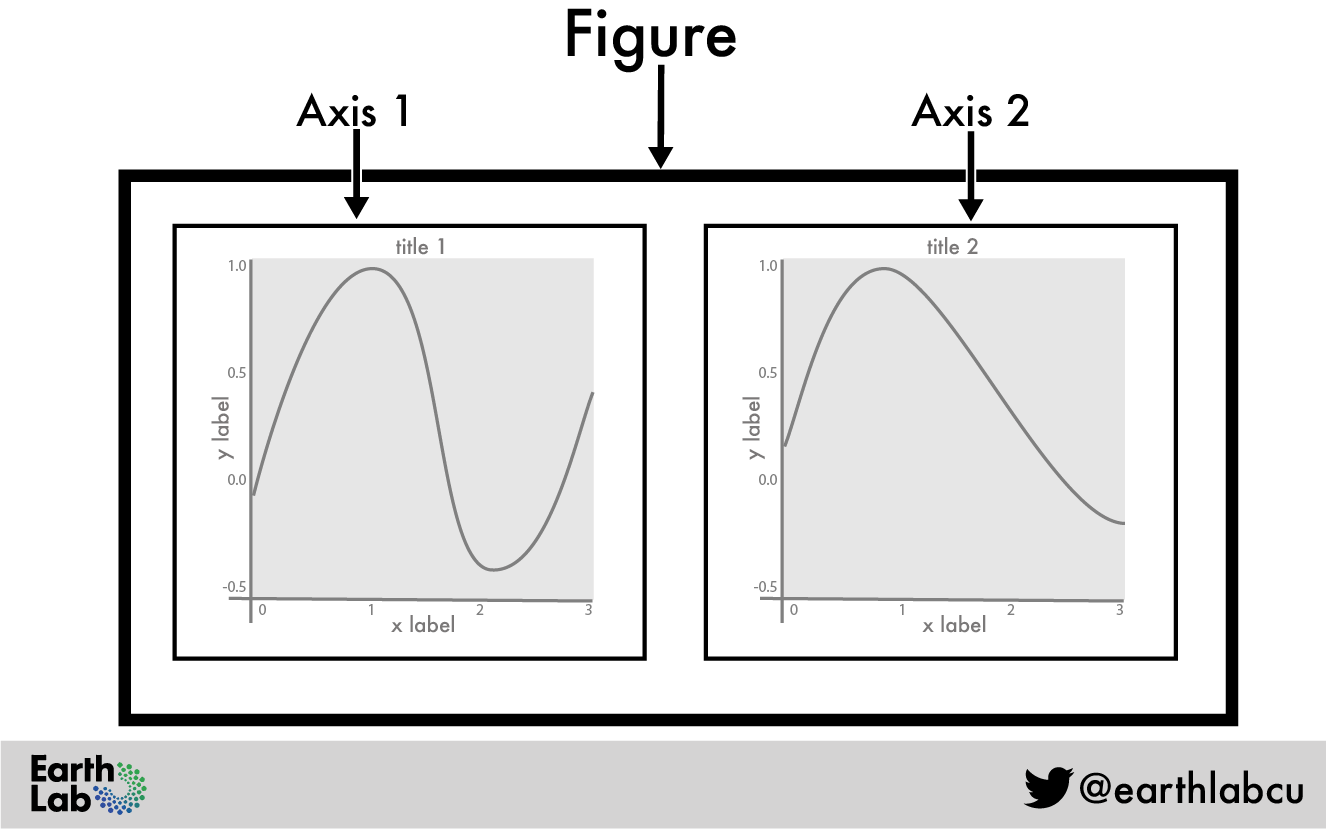
\includegraphics[height = 0.4\textheight]{Chapters/PNG/figureAxis.png}
\end{center}


\section{Creating a Figure}
\begin{prettyBox}{Figure Creation}{myblue}
\begin{itemize}
    \item A figure is created using the \texttt{figure()} function from the \texttt{pyplot} submodule.
    \item By default, Matplotlib starts with an implicit figure.
    \item Each additional call to \texttt{figure()} creates a new figure, so the total number of figures is :
        \begin{center}
            \boxed{\texttt{1 + (number of calls to figure())}}
        \end{center}
\end{itemize}
\end{prettyBox}

\vspace{0.5cm}


\section{Drawing A Plot}
\begin{prettyBox}{Plot}{myblue}
\texttt{plot()} is a function from the \texttt{pyplot} submodule used to draw a graph on the axis of a figure.\\[0.05cm] 
\texttt{plot(x, y, linestyle='-', linewidth=1.5, marker=None, markersize=6.0, color=auto, mfc=color, mec=color, label=None, alpha=1)}

\begin{itemize}
    \item \textbf{x}: A NumPy array representing the x-coordinates of the data points.
    \item \textbf{y}: A NumPy array representing the y-coordinates of the data points.
    \item \textbf{linestyle}: Optional parameter. Default is \texttt{'-'}. Specifies the style of the connecting line.
    \item \textbf{linewidth}: Optional parameter. Default is \texttt{1.5}. Controls the thickness of the line.
    \item \textbf{marker}: Optional parameter. Default is \texttt{None}. Defines the shape of markers placed at data points.
    \item \textbf{markersize}: Optional parameter. Default is \texttt{6.0}. Sets the size of the markers.
    \item \textbf{color}: Optional parameter. Default is \texttt{auto}. If not set, Matplotlib assigns a color automatically. Accepts color names, hex codes, and RGB(A) tuples.
    \item \textbf{mfc} (Marker Face Color): Optional parameter. Default is the same as \texttt{color}. Defines the fill color of the marker.
    \item \textbf{mec} (Marker Edge Color): Optional parameter. Default is the same as \texttt{color}. Defines the outline color of the marker.
    \item \textbf{label}: Optional parameter. Default is \texttt{None}. Specifies the legend label for the plot. Supports raw strings and LaTeX expressions using \texttt{\$ \$}.
    \item \textbf{alpha}: Optional parameter. Default is \texttt{1}. Controls the transparency of both lines and markers (1 = fully opaque, 0 = fully transparent).
\end{itemize}
\end{prettyBox}

\newpage

\begin{center}
    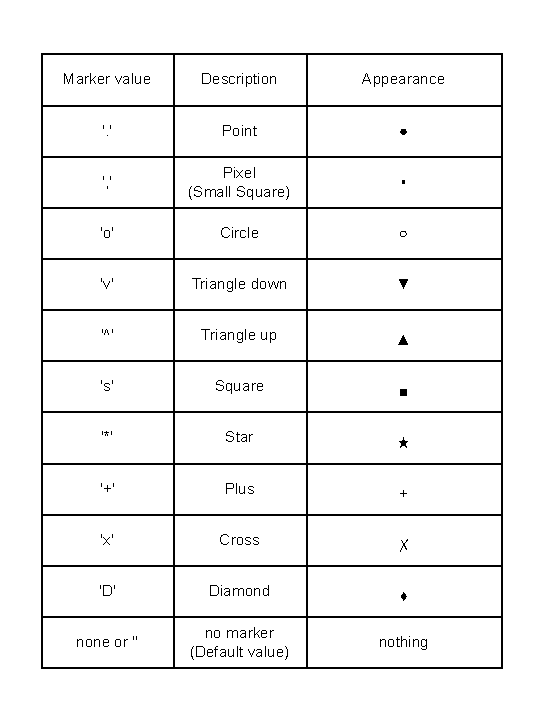
\includegraphics[height=0.6\textheight]{Chapters/PDF/marker.drawio.pdf}
\end{center}

\begin{center}
    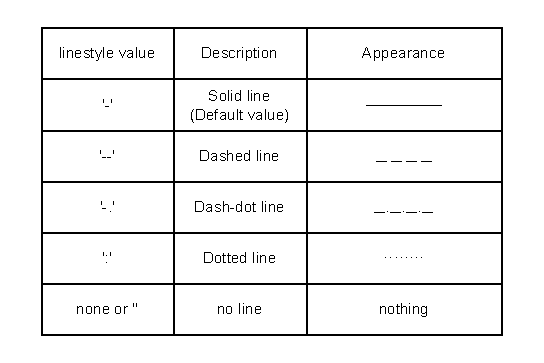
\includegraphics[height=0.35\textheight]{Chapters/PDF/linestyle.drawio.pdf}
\end{center}

\newpage

\section{Drawing a Single Point}
\begin{prettyBox}{Single Point}{myblue}
We can use either the \texttt{plot()} or \texttt{scatter()} function:
\begin{itemize}
    \item \texttt{plot(x, y, color=auto,linestyle='', marker, mfc=color, mec=color, alpha=1)}
    \item \texttt{scatter(x, y, color=auto, marker, c=color, edgecolors=color, alpha=1)}  
          Here, \texttt{c} is equivalent to \texttt{mfc}, and \texttt{edgecolors} is equivalent to \texttt{mec}.
\end{itemize}
\end{prettyBox}

\vspace{0.5cm}

\section{Graph Customization \& Display}
\begin{prettyBox}{Customization}{myblue}
\begin{itemize}
    \item \texttt{legend()}: Displays the labels of plotted elements (e.g., lines, scatter points) as a legend for the axis.
    \item \texttt{grid(visible=True)}: Toggles the grid on the axis. By default, the grid is off, but calling the function without arguments is equivalent to setting it to \texttt{True}.
    \item \texttt{title(label)}: Sets the title for the current axis.
    \item \texttt{suptitle(label)}: Sets the title for the current figure.
    \item \texttt{ylabel(label)}: Labels the y-axis.
    \item \texttt{xlabel(label)}: Labels the x-axis.
    \item \texttt{show()}: Renders and displays all created figures along with their content.
    \item \texttt{plt.savefig(fname)}: saves the figure in the given path fname , if fname doesn't have a file extension it will save it as png
\end{itemize}
\end{prettyBox}

\vspace{0.5cm}

\section{Subplot}
\begin{prettyBox}{Subplot}{myblue}
The \texttt{subplot()} function allows us to create multiple axes within the same figure by defining a grid layout.  

\texttt{subplot(nrows, ncols, index)}

\begin{itemize}
    \item \textbf{nrows}: Number of rows in the subplot grid.
    \item \textbf{ncols}: Number of columns in the subplot grid.
    \item \textbf{index}: The position of the subplot, starting from 1 (left to right, top to bottom).
\end{itemize}

Each call to \texttt{subplot()} activates a different subplot within the figure.  
\end{prettyBox}

\newpage
\textbf{\underline{Example}}\\[0.1cm]
\lstinputlisting[style=pythonstyle]{Chapters/Code/PLT/figure.py}

\newpage
\textbf{\underline{fig1}}\\[0.1cm]
\begin{center}
    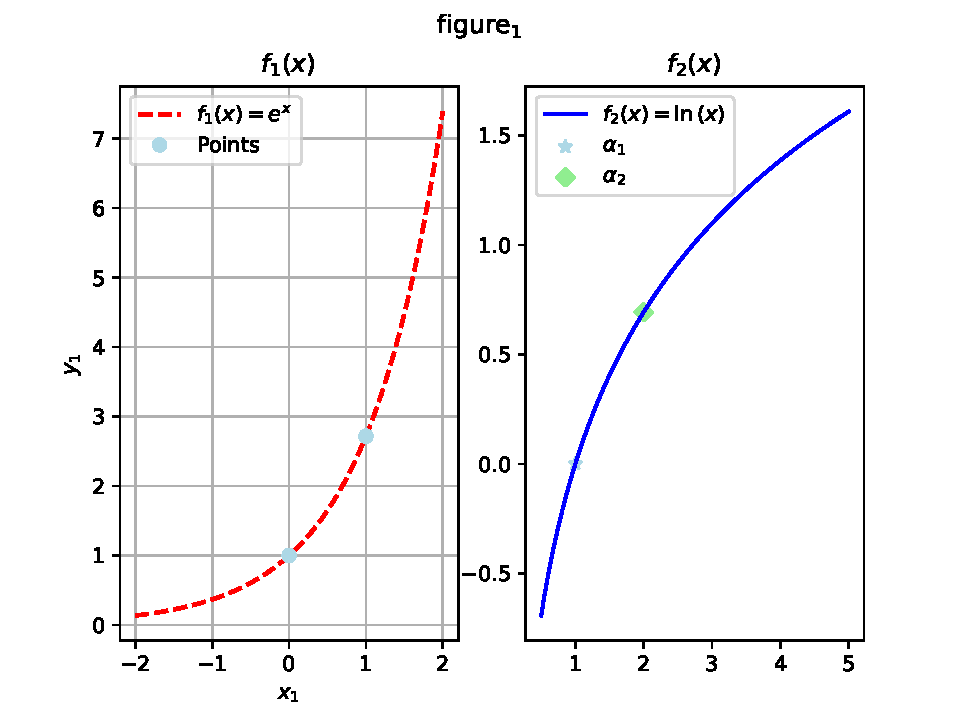
\includegraphics[height=0.35\textheight]{Chapters/Code/PLT/fig1.pdf}
\end{center}


\textbf{\underline{fig 2}}\\[0.1cm]
\begin{center}
    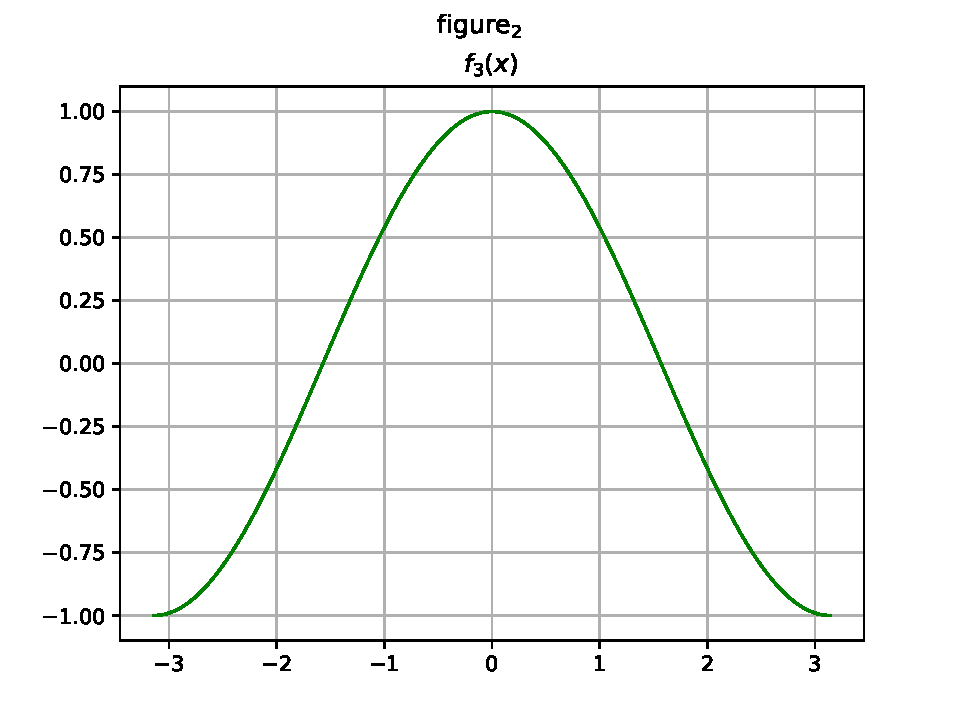
\includegraphics[height=0.35\textheight]{Chapters/Code/PLT/fig2.pdf}
\end{center}

\newpage

\begin{prettyBox}{Note}{red}
We can remove the \(x , y\) axes of an axis from showing by using the \texttt{plt.axis('off')} function.
\end{prettyBox}

\vspace{1cm}

\section{Drawing Tables}
\begin{prettyBox}{Table}{myblue}
To draw a table on an axis, we use the \texttt{table()} function, which returns a \texttt{Table} object.\\[0.1cm]
\texttt{the\_table = table(cellText, colLabels=None, rowLabels=None, cellLoc='right', fontsize=auto, colWidths=None, loc='bottom')}
\begin{itemize}
    \item \textbf{cellText}: A 2D list of strings that holds the content of each cell.
    \item \textbf{colLabels} (optional, default: \texttt{None}): A list of strings for the column headers.
    \item \textbf{rowLabels} (optional, default: \texttt{None}): A list of strings for the row headers.
    \item \textbf{cellLoc} (optional, default: \texttt{'right'}): Alignment of cell content. Possible values: \texttt{'right'}, \texttt{'left'}, \texttt{'center'}.
    \item \textbf{fontsize} (optional, default: \texttt{auto}): The font size of the table text.
    \item \textbf{colWidths} (optional): A list of floats representing the width of each column.
    \item \textbf{loc} (optional, default: \texttt{'bottom'}): The position of the table relative to the axes.
\end{itemize}

\vspace{0.15cm}

Some Function of \texttt{Table} object

\begin{itemize}
    \item \texttt{the\_table.auto\_set\_column\_width(col=None)} :  
        Adjusts the width of selected columns to fit their content.  
        \begin{itemize}
            \item \textbf{col} (optional, default: \texttt{None}): A list of integers representing the column indices to adjust.
        \end{itemize}

    \item \texttt{the\_table.scale(xscale, yscale)} :  
        Scales the table by adjusting cell padding.  
        \begin{itemize}
            \item \textbf{xscale} : Horizontal scaling factor.
            \item \textbf{yscale} : Vertical scaling factor.
        \end{itemize}

    \item \texttt{the\_table.auto\_set\_font\_size(scale=True)} :  
        Shrink font size until text fit in cell note that scaling padding with scale or calling the auto set columns width might override the behaviour
        of this function since text will always fit, and this behaviour is on by default.  
\begin{itemize}
    \item \textbf{scale} (optional , default = True) : boolean either True or False.
\end{itemize}

    \item \texttt{the\_table.set\_fontsize(size)} :  
        Manually sets the font size of the table text.
    \begin{itemize}
        \item \textbf{size} : float value. 
    \end{itemize}
   \end{itemize}
\end{prettyBox}

\newpage
\textbf{\underline{Example}}\\[0.1cm]
\lstinputlisting[style=pythonstyle]{Chapters/Code/PLT/tab.py}

\vspace{0.5cm}
\textbf{\underline{fig1}}\\[0.1cm]
\begin{center}
    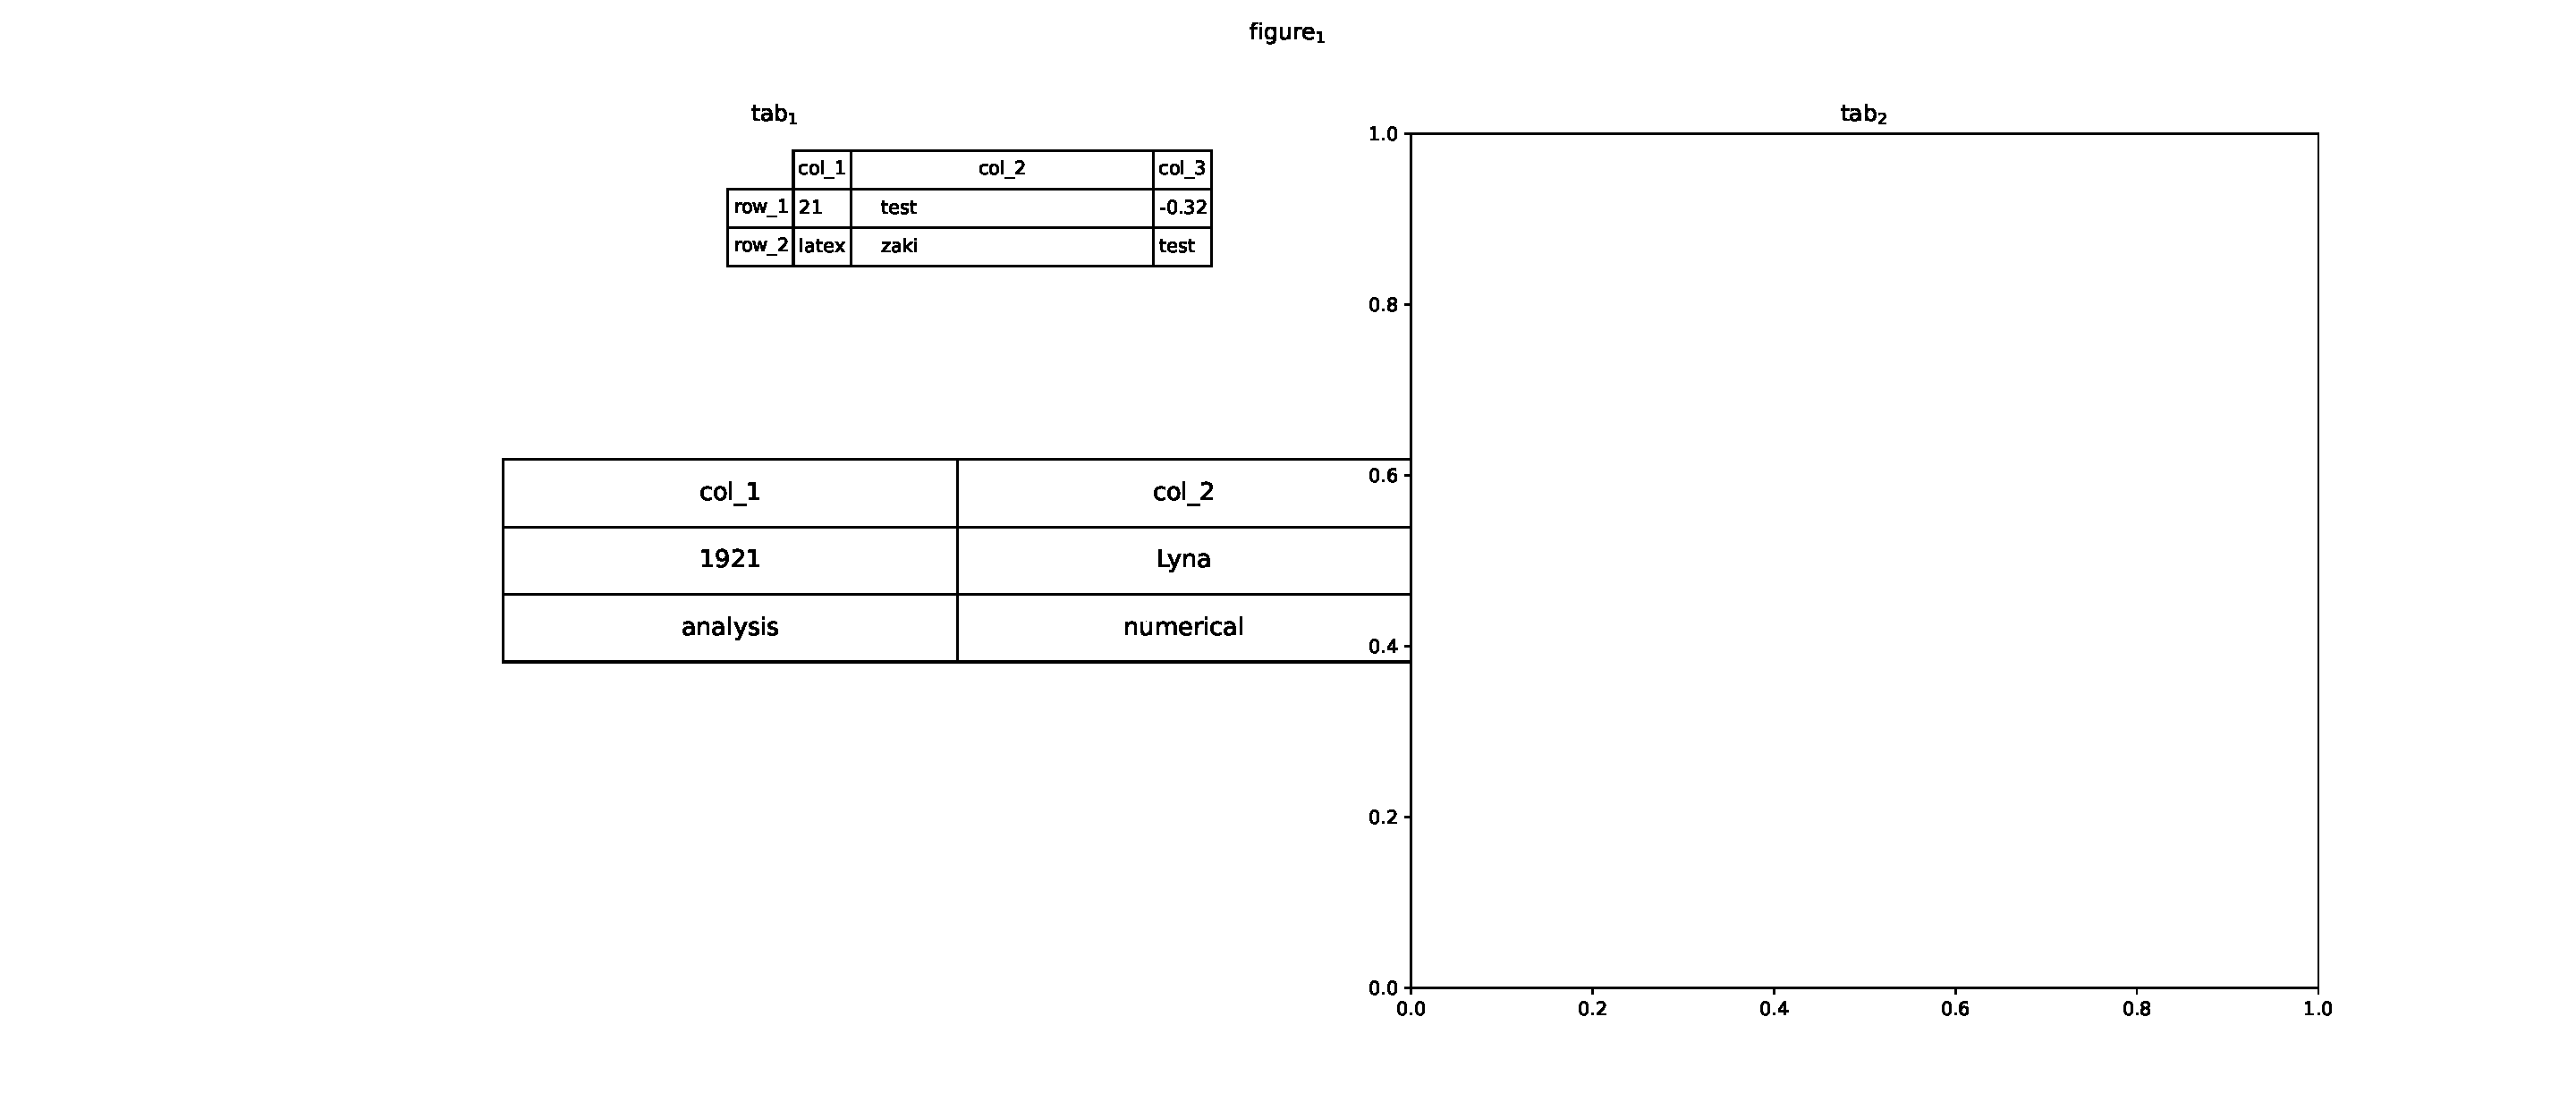
\includegraphics[height=0.35\textheight]{Chapters/Code/PLT/tab.pdf}
\end{center}



